% ---------- Payload ----------

Sizing a LASER-ablation deorbiting system involves a direct physical trade-off:
 the LASER must not destroy the debris through excessive heat input, 
 but must vaporise a very thin layer of its surface to create a propulsive plasma that slows the moving debris. 
 Thus, modifying the orbit of an object (debris) relies on converting the optical energy deposited by laser pulses into the mechanical energy of the plasma jet.

\subsection{LASER Ablation Propulsion}
When a high-intensity LASER beam strikes the surface of a material, 
the optical energy is absorbed instantaneously. 
The temperature of the surface layer rises so rapidly that it undergoes sudden sublimation and becomes a highly energetic plasma. 
This jet of matter is expelled at very high speeds. Under the physical law of conservation of matter, the ejection of matter generates a mechanical recoil force on the target object \cite{Vincent2011}.

\begin{figure}[H]
  \centering
  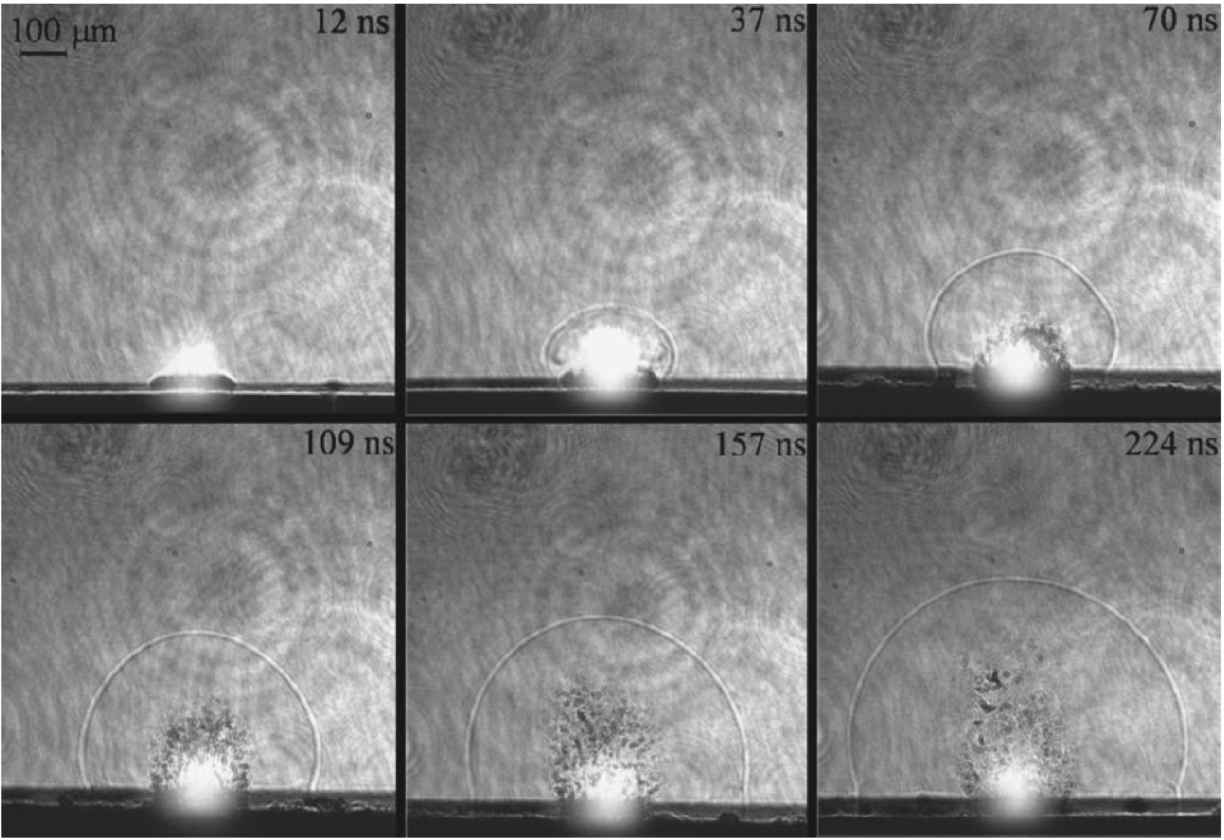
\includegraphics[width=0.8\textwidth,height=7cm,keepaspectratio]{ablation_laser.png}
  \caption{Images of the ablation propulsion process at different times during the laser--aluminium interaction for $\lambda = 1064 nm$ and $\tau = 5ns$. The propagation of the shock wave over time can be observed. \cite{Vincent2011}}
  \label{fig:ablation}
\end{figure}

\subsection{High-Power LASER Characteristics}
In this section, we describe the characteristics of our onboard high-power LASER. 
Selecting the high-power LASER is crucial: if its power or energy is unsuitable, 
it will probably not be possible to initiate the micropropulsion process at the surface of our target (debris).

\begin{enumerate}
    \item \textbf{Choice of LASER type:}\\
    We choose a pulsed LASER rather than a continuous-wave laser. 
    The factors determining this choice are summarised in the table below

    \begin{table}[H]
      \centering
      \caption{Comparison between continuous-wave and pulsed lasers.}
      \begin{tabular}{p{3.5cm} p{5.5cm} p{5.5cm}}
        \toprule
        \textbf{Characteristic} & \textbf{Continuous-wave laser } & \textbf{Pulsed laser} \\
        \midrule
        Effect on debris & Thermal melting  & Plasma ablation (mechanical rocket effect) \\
        Peak power & Equal to average power  & Several megawatts during the pulse \\
        Generated thrust & Almost zero at this power level & Optimal and directional \\
        Risks & High risk of breaking up the debris & Safe, targeted surface action \\
        \bottomrule
      \end{tabular}
    \end{table}

    \item \textbf{Required LASER parameters:}\\
    The wavelength of our high-power LASER is set to $\lambda = $\SI{1064}{\nano\metre} in the infrared, with a pulse duration of \textbf{nanoseconds (ns)}. This choice is primarily based on the absorption characteristics of the material making up our debris, namely aluminium (Al).

    For this CubeSat project using a $6U$ platform firing a LASER at short range, the optimal average power required for our small aluminium debris object, measuring \SIrange{1}{10}{\centi\metre} and weighing $1kg$ is approximately $1000W$. The choice of this operating power is deliberate and results from a specific trade-off validated by orbital mechanics and the physics of laser--matter interaction. The section on project feasibility discusses in detail the importance of reaching this optimal LASER ablation power.

    \begin{table}[H]
      \centering
      \small
      \caption{Ablation laser parameters.}
      \label{tab:laser_ablation}
      \begin{tabular}{p{6cm} p{6cm}}
        \toprule
        \textbf{Parameter} & \textbf{Value} \\
        \midrule
        Wavelength ($\lambda$) & \SI{1064}{\nano\metre} (infrared) \\
        Operating mode & Pulsed \\
        Pulse duration ($\tau$) & Nanosecond (ns) \\
        Average power ($P_{\text{moy}}$) & \SI{1000}{\watt} (\SI{1}{\kilo\watt}) \\
        Repetition rate ($f$) & \SI{3000}{\hertz} (\SI{2}{\kilo\hertz}) \\
        Pulse energy ($E_p$) & \SI{0.5}{\joule} \\
        Peak power ($P_{\text{crête}}$) & \SI{100}{\mega\watt} \\
        Ablation threshold fluence & \SIrange{1}{2}{\joule\per\centi\metre\squared} \\
        Optimal coupling fluence & \SI{5}{\joule\per\centi\metre\squared} \\
        \bottomrule
      \end{tabular}
    \end{table}
\end{enumerate}

\subsection{LiDAR for Detection}
To meet the imposed dimensional constraints, we favour a micro-LiDAR over a conventional LiDAR, which would entail higher mass and energy demands. The micro-LiDAR provides optical metrology of the debris: detection, relative position and relative velocity \cite{OpromollaNocerino}. It consists of three main elements:
\begin{itemize}
    \item The emission source, which in our case could be a VCSEL (Vertical Cavity Surface Emitting LASER). These are arrays of miniature semiconductor LASERs. The table below summarises the parameters we consider optimal for defining the LASER source of our micro-LiDAR.

    \begin{table}[H]
      \centering
      \small
      \caption{Micro-LiDAR laser parameters \cite{VCSEL1550_2023}.}
      \label{tab:lidar_laser}
      \begin{tabular}{p{3.3cm} p{4.7cm} p{6.5cm}}
        \toprule
        \textbf{Parameter} & \textbf{Specified value} & \textbf{Purpose in space} \\
        \midrule
        Wavelength & \SI{1550}{\nano\metre} & Prevents blinding by the ablation laser (\SI{1064}{\nano\metre}) \\
        Source type & Pulsed laser diode (InGaAs) & Robustness, extreme compactness \\
        Pulse duration & \SI{3}{\nano\second} & Millimetre-level ranging accuracy \\
        Frequency & \SI{20}{\kilo\hertz} & Smooth real-time target tracking \\
        Pulse energy & \SI{10}{\micro\joule} & Completely harmless to the debris \\
        Electrical power consumption & $\approx\SI{12}{\watt}$ & Fully suited to the constraints of a 6U CubeSat \\
        \bottomrule
      \end{tabular}
    \end{table}

    \item An ultrasensitive SPAD (Single Photon Avalanche Diode) detector. These detectors can detect a single returning photon. The table below summarises the parameters we consider optimal for selecting a suitable detector for our micro-LiDAR \cite{Pellegrini2006}.

    \begin{table}[H]
      \centering
      \small
      \caption{Micro-LiDAR SPAD detector parameters \cite{SPADReview2024}.}
      \label{tab:lidar_spad}
      \begin{tabular}{p{3.3cm} p{4.7cm} p{6.5cm}}
        \toprule
        \textbf{Parameter} & \textbf{Specified value} & \textbf{Purpose in space} \\
        \midrule
        Detector type & SPAD InGaAs/InP & Sensitive at \SI{1550}{\nano\metre}, single-photon detection \\ % to be verified
        Detection efficiency & $\approx\SI{20}{\percent}$ at \SI{1550}{\nano\metre} & Detect the weak signal backscattered by the debris \\ % to be verified
        Timing jitter (\textit{jitter}) & $\approx\SI{200}{\pico\second}$ & Range resolution of a few centimetres \\ % to be verified
        Dark count rate & $\approx\SI{10}{\kilo\hertz}$ (cooled detector) & Limit noise to maintain a good signal-to-noise ratio \\ % to be verified
        Operating mode & Gated (\textit{gated}), synchronised with the pulse & Reduce noise and power consumption \\ % to be verified
        \bottomrule
      \end{tabular}
    \end{table}

    \item MEMS (Micro-Electro-Mecanical System) micromirrors. These oscillating micromirrors are etched into silicon to steer the beam without heavy mechanical components. The table below summarises the parameters we consider optimal for selecting the mirror assembly for our micro-LiDAR \cite{Shea2006}.

    \begin{table}[H]
      \centering
      \small
      \caption{Micro-LiDAR oscillating MEMS micromirror parameters \cite{Liu2022}.}
      \label{tab:lidar_mems}
      \begin{tabular}{p{3.3cm} p{4.7cm} p{6.5cm}}
        \toprule
        \textbf{Parameter} & \textbf{Specified value} & \textbf{Purpose in space} \\
        \midrule
        Scanning mechanism & Resonant MEMS micromirror & Scene scanning without bulky mechanical components \\ % to be verified
        Mirror diameter & $\approx\SI{1}{\milli\metre}$ & Trade-off between optical aperture and resonant frequency \\ % to be verified
        Optical scan angle & $\pm\SI{10}{\degree}$ & Cover the field of view required for target acquisition \\ % to be verified
        Resonant frequency & $\approx\SI{1}{\kilo\hertz}$ & Scan rate compatible with real-time tracking \\ % to be verified
        Electrical power consumption & Less than $\SI{1}{\watt}$ & Compatible with the power budget of a 6U CubeSat \\ % to be verified
        \bottomrule
      \end{tabular}
    \end{table}
\end{itemize}

